\documentclass[11pt,a4paper]{article}
\usepackage[hyperref]{naaclhlt2019}
\usepackage{times}
\usepackage{latexsym}
\usepackage{xspace}
\usepackage{multirow}
\usepackage{url}
\usepackage{booktabs}
\usepackage{tikz,tikz-qtree}
\usepackage{pgfplots}
\usepackage{amssymb}
\usepackage{xfrac}
\usepackage{graphicx}
\usepackage{tablefootnote}
\usepackage{amsmath}
\usepackage{enumitem}
\pgfplotsset{compat=1.14}

\newcommand\BibTeX{B{\sc ib}\TeX}

\aclfinalcopy % comment this when submitting the paper
%\def\aclpaperid{***} %  Enter the acl Paper ID here

%\setlength\titlebox{5cm}
% You can expand the titlebox if you need extra space
% to show all the authors. Please do not make the titlebox
% smaller than 5cm (the original size); we will check this
% in the camera-ready version and ask you to change it back.

\definecolor{g-red}{HTML}{DB4437}
\definecolor{g-blue}{HTML}{4285F4}
\definecolor{g-green}{HTML}{0F9D58}
\definecolor{g-yellow}{HTML}{F4B400}
\definecolor{g-orange}{HTML}{FF9800}
\definecolor{g-grey}{HTML}{9E9E9E}

\setlength{\tabcolsep}{0.3em}

\usepackage{todonotes}


\newcounter{mw}
\newcommand{\mw}[1]{%
\refstepcounter{mw}%
{%
\todo[color=orange, size=\footnotesize]{%
[\textbf{mw:\themw}] #1}%
}}%

\newcounter{jd}
\newcommand{\jd}[1]{%
\refstepcounter{jd}%
{%
\todo[color=green, size=\footnotesize]{%
[\textbf{jd:\thekt}] #1}%
}}%

\newcounter{kl}
\newcommand{\kl}[1]{%
\refstepcounter{kl}%
{%
\todo[color=magenta, size=\footnotesize]{%
[\textbf{kl:\thekl}] #1}%
}}%

\newcommand\bertbase{BERT$_{\small \textsc{BASE}}$\xspace}
\newcommand\bertlarge{BERT$_{\small \textsc{LARGE}}$\xspace}

\title{Bert \& TextCNN on SemEval-2017 Task4 subTask A: Sentiment Analysis in twitter}

\author{Huiqiang Jiang \\
  {\tt \{1801210840\}@pku.edu.cn} \\}

\date{}

% REMOVE THIS IN THE FINAL COPY!
% \hypersetup{draft}

\begin{document}
\maketitle
\begin{abstract}
  In this paper, we present two deep-learning models that competed at SemEval-2017 Task 4 "Sentiment Analysis in Twitter subTask A". We used Text Convolutional Neural Network (TextCNN), on encoder end using a pre-trained word embeddings on a big collection of Twitter from RepLab 2013 Dataset. Also, we using a text processing tool build by DataStories which performs tokenization, word normalization, segmentation, and spell correction. And we also evaluation in Bert and some traditional machine learning like logistic regression(LR), Support Vector Machines(SVM). The evaluation shows that embedding, text processor is most important, and neural network model better than traditional machine learning model. We achieve a 69.39\% Recall score on Task A,  Macro-F1 is 69.91\%, accuracy is 70.03\%. Every score is better than the rank 1 in the competition. In the future, we want to combine the TextCNN with Bert.  All code is available to the research community.
\end{abstract}

\section{Introduction}

Sentiment Analysis is a typical task in Natural Language Processing (NLP) domain. It is easy to start with some very simple method (e.g. positive - negative words counting). But If you want to get a good result, It is difficult. Because Twitter dataSet is informal and creative writing style. It means that you will encounter lots of out-of-vocabulary (OOV) situation. So maybe embedding is a very important point in the task. The practical applications of this task are wide, from personalized recommendation, chatbot, to public opinion monitoring(e.g. Presidential debates, World Cup, etc.).

In the last few years, deep learning techniques have significantly out-performed traditional methods in several NLP tasks,  and sentiment analysis is no exception to this trend. Especially Bert published on last year. Two of the most popular deep learning techniques for sentiment analysis are TextCNNs and Transform model like Bert. In this paper, we evaluation both two model.

In this paper, we present two deep-learning systems that competed at SemEval-2017 Task 4. Our first model base on a single-layer CNN model, equipped with 3 filters. The other model base on Bert which is a pre-training and fine-tuning model by the multi-layer transform.

\begin{itemize}
  \item  We evaluation this task in some traditional model, like SVM, LR. In this model, we get some decent result. We also used a text processor to change text format, like change `HTTP://' to `$<$url$>$'. It reduces the bag of word size, and reduce the out-of-vocabulary (OOV) situation.
  \item A pre-train embedding basing on RepLab 2013 Dataset. And we train this embedding in two way, word2vec and fastText. We find that the model pre-train by fastText work is better than pre-training by word2vec in LogisticRegression. So we choose the embedding by fastText as encoder tools.
  \item And we train model in textCNN \& Bert. we also evaluate the effect of pad position. All code can be found in github.\footnote{github.com/iofu728/SemEval2017-Task4-SentimentAnalysis.}
\end{itemize}


\section{System Description}
In this section, we describe our text processor and illustrate how we leverage pre-training word embedding and how to encode in our model. 
\begin{figure*}[t]
    \begin{center}
        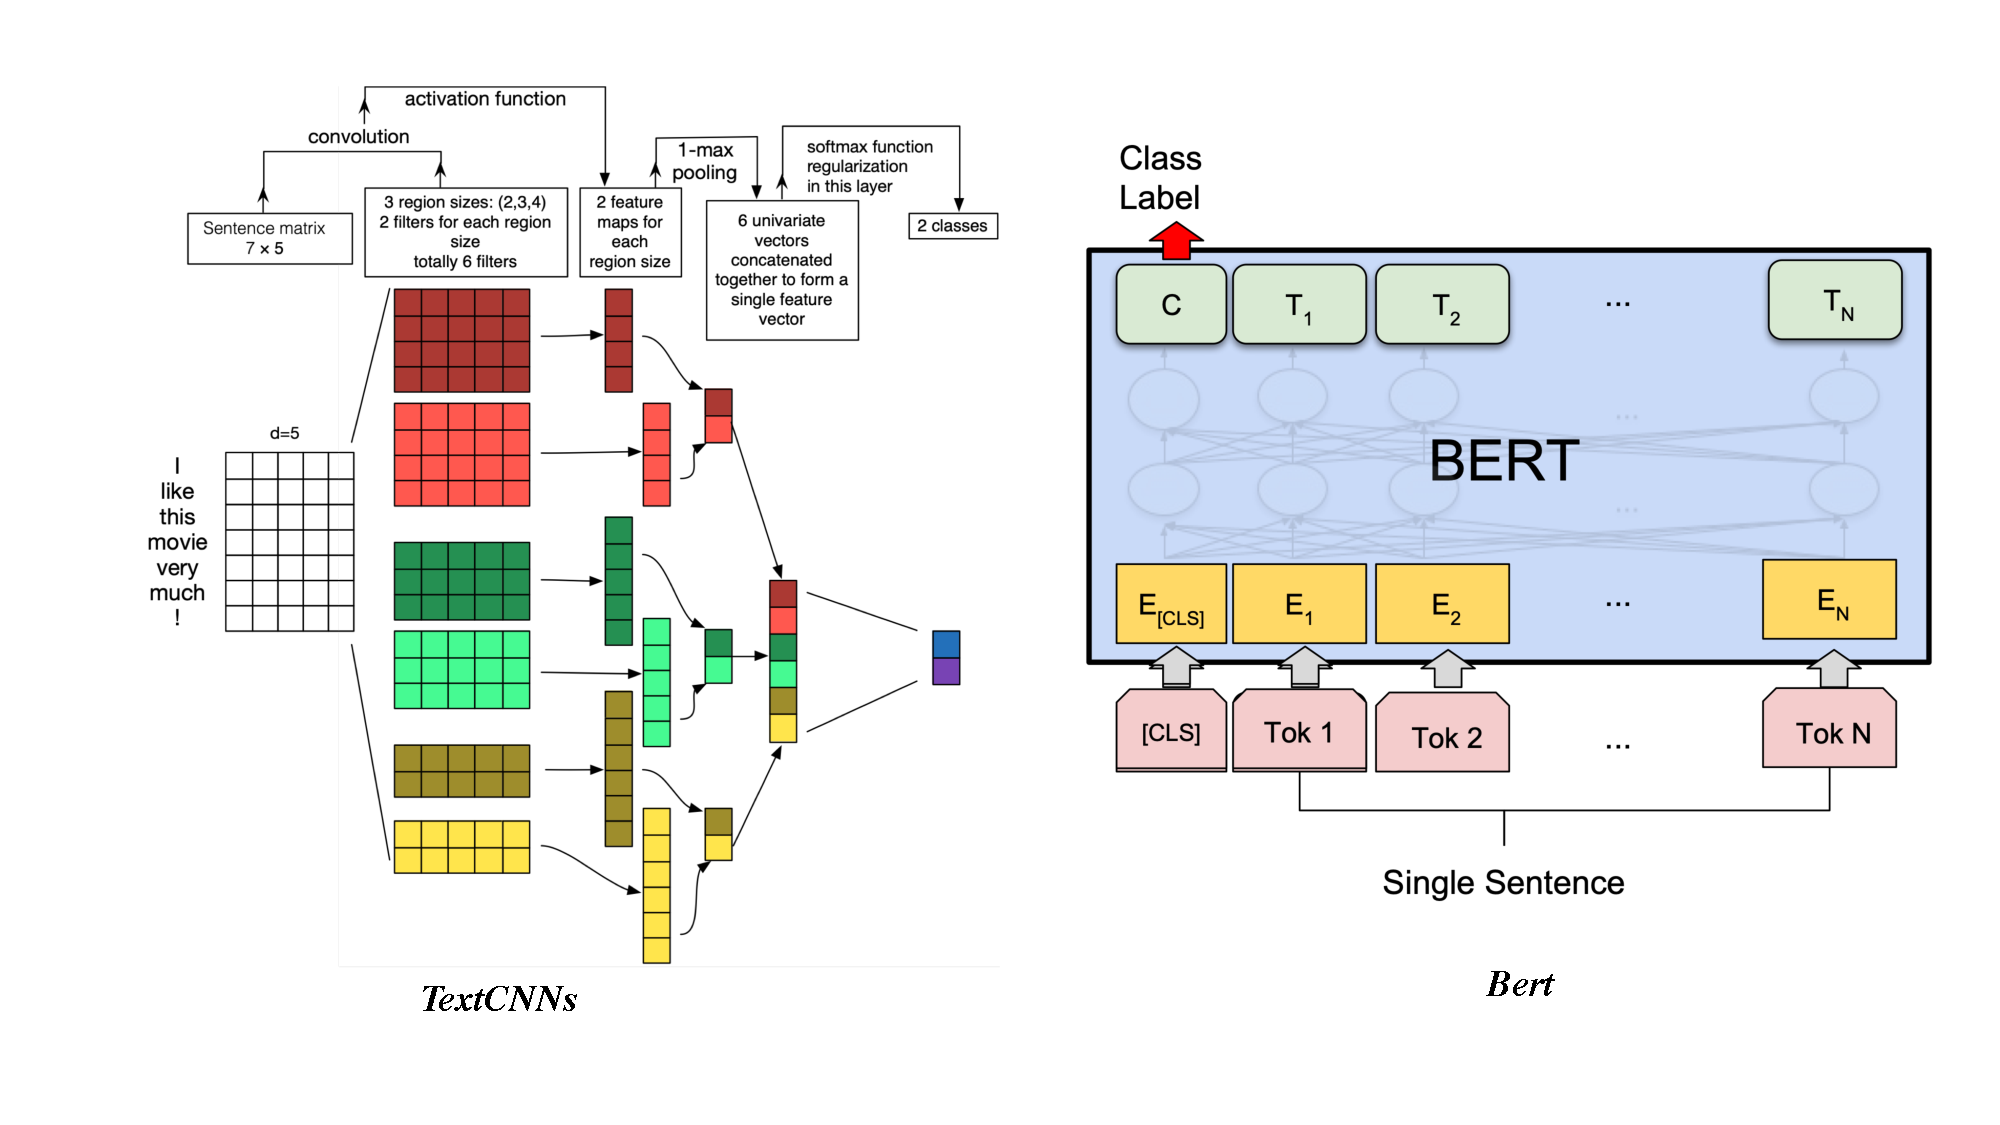
\includegraphics[width=\textwidth]{figures/figure.pdf}
    \end{center}
    \caption{Two model in this paper, TextCNN \& Bert}
    \label{fig:model}
\end{figure*}

    
\subsection{Text Processor}
The text processor reference by DataStroies \cite{biaziotis2017datastories}\footnote{github.com/cbaziotis/ekphrasis}. In this processor, we change emoji to a semantic word, change URL to label `$<$url$>$'. And we also lowercase all words and do some simple spell correction. This work can reduce the OOV situation. Before using the text processor, the ratio of OOV is 76.75\%(135619/177692). The ration of OOV using the text processor is 9.60\%(4491/45578). From this data, the text processing also reduces the word num.

After that, we alignment the sentences to max sentences line. In this processing, we add the pad to before first, after first, before the last one, after the lastest one respectively.

\subsection{Pre-training Embedding}

we pre-training the word embedding obtained from RepLab 2013 Dataset \cite{replab2013overview}\footnote{nlp.uned.es/replab2013/} about 9GB data. We train for word2vec \& fastText, having text processor, no text processor and respectively evaluation in LogisticRegression model. 


\subsection{TextCNN}

We first test in TextCNN model.  Its architecture is almost identical to CNN.  The input of the network are the tweets, which are tokenized into words which disposed of by text processor.  And each word is encoded by a word vector representation, i.e. a word embedding.  We also follow add zero-padding strategy such that all tweets have the same matrix dimension $X \in \mathbb{R}^{s'\times d}$, where we chose $s'=MaxSen.$=64(using TextProcessor)/35(no TextProcessor).  We then apply several convolution operations of various sizes to this matrix.  A single convolution involves a filtering matrix $w \in \mathbb{R}^{h\times d}$ where $h$ is the size of the convolution, meaning the number of words it spans.  The convolution operation is defined as 

\begin{eqnarray}
c_i &=& f \left( \sum_{j,k} w_{j,k} \left(X_{[i:i+h-1]} \right)_{j,k} + b \right)
\end{eqnarray}

where $b \in \mathbb{R}$ is a bias term and f(x) is a non-linear function, which we chose to be the `relu' function.  The output $c \in \mathbb{R}^{s'-h+1}$ is, therefore, a concatenation of the convolution operator over all possible window of words in the tweet. We can use multiple filtering matrices to learn different features, and additionally, we can use multiple convolution sizes to focus on smaller or larger regions of the tweets.  In practice, we used the filter size $[6,7,8]$ and we used a total of 256 filtering matrices for each filter size.\\

\subsection{Bert}

\begin{table*}[htbp!] % here top bottom page (! = remove further restrictions)
    \centering
    \begin{tabular}{llccccccc}
    \midrule
    Embedding Model  &  Text Processor          & Recall         & Precision       & Macro-F1        & Accuracy & Pos. &Neu. & Neg.\\
    \midrule
    no        & no           & 45.70   & 43.12     & 44.38    & 48.18    & 43.03 & \bf74.68    & 11.66 \\
    word2Vec  & no           & 44.87   & 42.48     & 43.65    & 51.37    & 60.81    & 57.27    & 9.37  \\
    fastText  & no           & 43.87   & 42.04     & 42.93    & 46.60    & 44.97    & 72.93    & 8.21  \\
    no        & ekphrasis    & 61.07   & 62.15     & 61.61    & 62.34 & \bf64.00    & 64.83    & 57.63 \\
    word2vec  & ekphrasis    & 61.49   & 62.35     & 61.92 & \bf64.37    & 62.52    & 68.72    & 55.80 \\
    fastText  & ekphrasis & \bf62.67 & 6\bf4.07 & \bf63.36    & 63.81    & 63.03    & 61.58 & \bf67.60 \\
    \bottomrule
    \end{tabular}
\caption{Comparison between different Embedding mode \& Text Processor using LibLinear logistic regression model on subtask A data (in \%)}
\label{tab:embedding}
\end{table*}

\begin{table*}[htbp!] % here top bottom page (! = remove further restrictions)
    \centering
    \begin{tabular}{rl}
    \midrule
        Sentences1:     &\textbf{\underline{Indian Mi Fans}}. Are Are Are \textbf{\underline{you}} ok? \\
        Sentences2:     &\textbf{\underline{Indian Mi Fans}}. Are \textbf{\underline{you}} ok? \\ 
        Before entity1: &\begin{scriptsize}[PAD] [PAD] \end{scriptsize} \textbf{\underline{Indian Mi Fans}}.  Are Are Are \textbf{\underline{you}} ok? \\
                        &\begin{scriptsize}[PAD] [PAD] [PAD] [PAD] \end{scriptsize}  \textbf{\underline{Indian Mi Fans}}. Are \textbf{\underline{you}} ok? \\
        After entity1:  &\textbf{\underline{Indian Mi Fans}}. \begin{scriptsize}[PAD] [PAD] \end{scriptsize} Are Are Are \textbf{\underline{you}} ok?\\
                        &\textbf{\underline{Indian Mi Fans}}. \begin{scriptsize}[PAD] [PAD] [PAD] [PAD] \end{scriptsize}  Are \textbf{\underline{you}} ok?\\
        Before entity2: &\textbf{\underline{Indian Mi Fans}}.  Are Are Are \begin{scriptsize}[PAD] [PAD] \end{scriptsize} \textbf{\underline{you}} ok? \\
                        &\textbf{\underline{Indian Mi Fans}}. Are \begin{scriptsize}[PAD] [PAD] [PAD] [PAD] \end{scriptsize}  \textbf{\underline{you}} ok? \\
        After entity2:  &\textbf{\underline{Indian Mi Fans}}. Are Are Are \textbf{\underline{you}} ok? \begin{scriptsize}[PAD] [PAD] \end{scriptsize} \\
                        &\textbf{\underline{Indian Mi Fans}}. Are \textbf{\underline{you}} ok? \begin{scriptsize}[PAD] [PAD] [PAD] [PAD] \end{scriptsize}  \\
    \bottomrule
    \end{tabular}
\caption{Pad example (MAX sentences size = 12)}
\label{tab:model}
\end{table*}

BERT is one of the key innovations in the recent progress of contextualized representation learning \cite{peters2018deep,howard2018universal,radford2018improving,devlin2018bert}.
The idea behind the progress is that even though the word embedding layer (in a typical neural network for NLP) is trained from large-scale corpora, training a wide variety of neural architectures that encode contextual representations only from the limited supervised data on end tasks is insufficient.
Unlike ELMo \cite{peters2018deep} and ULMFiT \cite{howard2018universal} that are intended to provide additional features for a particular architecture that bears human's understanding of the end task, BERT adopts a fine-tuning approach that requires almost no specific architecture for each end task. This is desired as an intelligent agent should minimize the use of prior human knowledge in the model design. Instead, it should learn such knowledge from data. BERT has two parameter intensive settings: 

\begin{itemize}
    \item {\bf \bertbase}: L=12, H=768, A=12, Total Parameters=110M
    \item {\bf \bertlarge}: L=24, H=1024, A=16, Total Parameters=340M
\end{itemize}

\section{Experiments}
\label{sec:experiments}

In this section, we evaluate in embedding, text processor, model.

\subsection{Embedding}
\label{sec:embedding}

Word embedding almost the important thing in NLP task. So we take some word embedding method and train dataSet to tune the effect of word embedding.

First of all, the train dataSet of competition is so small that the effect of training word embedding is bad. So we import some outer dataSet to optimization the effect of word embedding. The domain of our task is about scientific papers. So, we load dataset on RepLab 2013 Dataset. 

We also do some work on different word embedding methods, like word2vec, fastText. FatsText do the best job in our experiment. Bert doesn't have a good effect on our task. We think it may be caused by the difficult word style between pre-train model and twitter dataSet.

\subsection{TextCNN}
\label{sec:textCNN}

\begin{table*}[htbp!] % here top bottom page (! = remove further restrictions)
    \centering
    \begin{tabular}{llccccccc}
    \midrule
    Text Position  &  Pad position          & Recall         & Precision       & Macro-F1        & Accuracy & Pos. &Neu. & Neg.\\
    \midrule
    no   & before 0  & 61.39 & 49.50 & 54.81 & 57.57 & 41.76 & \bf85.10 & 21.64 \\
    no  & after 1   & 64.77 & 51.93 & 57.64 & 61.10 & 53.97 & 82.90 & 18.91 \\
    no  & before -1 & 63.08 & 52.18 & 57.11 & 59.20 & 45.72 & 83.17 & 27.64 \\
    no  & after end & 62.05 & 57.54 & 59.71 & 63.00 & 57.58 & 76.85 & 38.19 \\
    ekphrasis   & before 0  & 61.61 & \bf65.62 & 63.55 & 63.70 & 69.12 & 56.54 & \bf71.21 \\
    ekphrasis  & after 1   & \bf66.70 & 59.73 & 63.02 & 66.27 & 60.88 & 80.92 & 37.37 \\
    ekphrasis  & before -1 & 64.71 & 61.61 & 63.12 & 65.23 & \bf77.62 & 61.70 & 45.51 \\
    ekphrasis  & after end & 65.36 & 62.37 & \bf63.83 & \bf66.93 & 70.02 & 71.12 & 45.98 \\

    \bottomrule
    \end{tabular}
\caption{Comparison between different Text Processor \& Pad position using TextCNN model on subtask A data (in \%)}
\label{tab:text_cnn}
\end{table*}

\section{BERT}
\label{sec:bert}

We introduce BERT and  its detailed implementation in this section. We first cover the model architecture and the input representation for BERT. We then introduce the pre-training tasks, the core innovation in this paper, in Section~\ref{sec:pretraining_tasks}. The pre-training procedures, and fine-tuning procedures are detailed in Section~\ref{sec:pretraining_procedure} and~\ref{sec:finetuning_procedure}, respectively. Finally, the differences between BERT and OpenAI GPT are discussed in Section~\ref{sec:comparing_bert_and_openai}.

\subsection{Model Architecture}
\label{sec:model_architecture}

BERT's model architecture is a multi-layer bidirectional Transformer encoder based on the original implementation described in \citet{vaswani-etal:2017:_atten} and released in the {\tt tensor2tensor} library.\footnote{https://github.com/tensorflow/tensor2tensor} Because the use of Transformers has become ubiquitous recently and our implementation is effectively identical to the original, we will omit an exhaustive background description of the model architecture and refer readers to \citet{vaswani-etal:2017:_atten} as well as excellent guides such as ``The Annotated Transformer.''\footnote{http://nlp.seas.harvard.edu/2018/04/03/attention.html}

In this work, we denote the number of layers (i.e., Transformer blocks) as $L$, the hidden size as $H$, and the number of self-attention heads as $A$. In all cases we set the feed-forward/filter size to be $4H$, i.e., 3072 for the $H=768$ and 4096 for the $H=1024$. We primarily report results on two model sizes:

\begin{itemize}
\item {\bf \bertbase}: L=12, H=768, A=12, Total Parameters=110M
\item {\bf \bertlarge}: L=24, H=1024, A=16, Total Parameters=340M
\end{itemize}

\bertbase was chosen to have an identical model size as OpenAI GPT for comparison purposes. Critically, however, the BERT Transformer uses bidirectional self-attention, while the GPT Transformer uses constrained self-attention where every token can only attend to context to its left. We note that in the literature the bidirectional Transformer is often referred to as a ``Transformer encoder'' while the left-context-only version is referred to as a ``Transformer decoder'' since it can be used for text generation. The comparisons between BERT, OpenAI GPT and ELMo are shown visually in Figure~\ref{fig:BERT_comparisons}.


\subsection{Input Representation}
\label{sec:input_representation}


\begin{figure*}[tbh]
\begin{center}
\hspace{-0.2in}
\includegraphics[width=400px]{figures/Input_Emebeddings.pdf}
\end{center}
\caption{BERT input representation. The input embeddings is the sum of the token embeddings, the segmentation embeddings and the position embeddings.}
\label{tab:input_emebeddings}
\end{figure*}

Our input representation is able to unambiguously represent both a single text sentence or a pair of text sentences (e.g., [Question, Answer]) in one token sequence.\footnote{Throughout this work, a ``sentence'' can be an arbitrary span of contiguous text, rather than an actual linguistic sentence. A ``sequence'' refers to the input token sequence to BERT, which may be a single sentence or two sentences packed together.} For a given token, its input representation is constructed by summing the corresponding token, segment and position embeddings. A visual representation of our input representation is given in Figure~\ref{tab:input_emebeddings}. 

The specifics are:

\begin{itemize} 
\item We use WordPiece embeddings \cite{wu-etal:2016:_googl} with a 30,000 token vocabulary. We denote split word pieces with {\tt \#\#}.
\item We use learned positional embeddings with supported sequence lengths up to 512 tokens.
\item The first token of every sequence is always the special classification embedding ({\tt [CLS]}). The final hidden state (i.e., output of Transformer) corresponding to this token is used as the aggregate sequence representation for classification tasks. For non-classification tasks, this vector is ignored.
\item Sentence pairs are packed together into a single sequence. We differentiate the sentences in two ways. First, we separate them with a special token ({\tt [SEP]}). Second, we add a learned sentence {\tt A} embedding to every token of the first sentence and a sentence {\tt B} embedding to every token of the second sentence.
\item For single-sentence inputs we only use the sentence {\tt A} embeddings.
\end{itemize}

\subsection{Pre-training Tasks}
\label{sec:pretraining_tasks}

Unlike \citet{peters-etal:2018:_deep} and \citet{radford-etal:2018}, we do not use traditional left-to-right or right-to-left language models to pre-train BERT. Instead, we pre-train BERT using two novel unsupervised prediction tasks, described in this section.

\subsubsection{Task \#1: Masked LM}
Intuitively, it is reasonable to believe that a deep bidirectional model is strictly more powerful than either a left-to-right model or the shallow concatenation of a left-to-right and right-to-left model. Unfortunately, standard conditional language models can only be trained left-to-right {\it or} right-to-left, since bidirectional conditioning would allow each word to indirectly ``see itself'' in a multi-layered context.

In order to train a deep bidirectional representation, we take a straightforward approach of masking some percentage of the input tokens at random, and then predicting only those masked tokens. We refer to this procedure as a ``masked LM'' (MLM), although it is often referred to as a {\it Cloze} task in the literature~\cite{taylor:1953:_cloze}. In this case, the final hidden vectors corresponding to the mask tokens are fed into an output softmax over the vocabulary, as in a standard LM. In all of our experiments, we mask 15\% of all WordPiece tokens in each sequence at random. In contrast to denoising auto-encoders \cite{vincent:2008}, we only predict the masked words rather than reconstructing the entire input.

Although this does allow us to obtain a bidirectional pre-trained model, there are two downsides to such an approach. The first is that we are creating a mismatch between pre-training and fine-tuning, since the {\tt [MASK]} token is never seen during fine-tuning. To mitigate this, we do not always replace ``masked'' words with the actual {\tt [MASK]} token. Instead, the training data generator chooses 15\% of tokens at random, e.g., in the sentence {\tt {\small my dog is hairy}} it chooses {\tt {\small hairy}}. It then performs the following procedure:
\begin{itemize}
\item Rather than {\em always} replacing the chosen words with {\tt [MASK]}, the data generator will do the following:
\item 80\% of the time: Replace the word with the {\tt [MASK]} token, e.g., {\tt {\small my dog is hairy $\rightarrow$ my dog is [MASK]}}
\item 10\% of the time: Replace the word with a random word, e.g., {\tt {\small my dog is hairy $\rightarrow$ my dog is apple}}
\item 10\% of the time: Keep the word unchanged, e.g., {\tt {\small my dog is hairy $\rightarrow$ my dog is hairy}}. The purpose of this is to bias the representation towards the actual observed word.
\end{itemize}

The Transformer encoder does not know which words it will be asked to predict or which have been replaced by random words, so it is forced to keep a distributional contextual representation of {\it every} input token. Additionally, because random replacement only occurs for 1.5\% of all tokens (i.e., 10\% of 15\%), this does not seem to harm the model's language understanding capability. 

The second downside of using an MLM is that only 15\% of tokens are predicted in each batch, which suggests that more pre-training steps may be required for the model to converge. In Section~\ref{sec:num_training_steps} we demonstrate that MLM does converge marginally slower than a left-to-right model (which predicts every token), but the empirical improvements of the MLM model far outweigh the increased training cost.

\subsubsection{Task \#2: Next Sentence Prediction}
Many important downstream tasks such as Question Answering (QA) and Natural Language Inference (NLI) are based on understanding the {\it relationship} between two text sentences, which is not directly captured by language modeling. In order to train a model that understands sentence relationships, we pre-train a binarized {\it next sentence prediction} task that can be trivially generated from any monolingual corpus. Specifically, when choosing the sentences {\tt A} and {\tt B} for each pre-training example, 50\% of the time {\tt B} is the actual next sentence that follows {\tt A}, and 50\% of the time it is a random sentence from the corpus. For example:
\begin{align*}
\text{Input\;} &= \text{\tt {\scriptsize [CLS] the man went to [MASK] store [SEP]}} \\ 
& \text{\tt {\scriptsize \;\;\;\;\;\;\;he bought a gallon [MASK] milk [SEP]}}\\
\text{Label} &= \text{\tt {\scriptsize IsNext}} \\
\\
\text{Input\;} &= \text{\tt {\scriptsize [CLS] the man [MASK] to the store [SEP]}}\\
&\text{\tt {\scriptsize \;\;\;\;\;\;\;penguin [MASK] are flight \#\#less birds [SEP]}}\\
\text{Label} &= \text{\tt {\scriptsize NotNext}}
\end{align*}
We choose the {\tt {\small NotNext}} sentences completely at random, and the final pre-trained model achieves 97\%-98\% accuracy at this task. Despite its simplicity, we demonstrate in Section~\ref{sec:task_ablation} that pre-training towards this task is very beneficial to both QA and NLI.

\subsection{Pre-training Procedure}
\label{sec:pretraining_procedure}

The pre-training procedure largely follows the existing literature on language model pre-training. For the pre-training corpus we use the concatenation of BooksCorpus (800M words) \cite{zhu:2015} and English Wikipedia (2,500M words). For Wikipedia we extract only the text passages and ignore lists, tables, and headers. It is critical to use a document-level corpus rather than a shuffled sentence-level corpus such as the Billion Word Benchmark \cite{chelba-etal:2013:_one} in order to extract long contiguous sequences.

To generate each training input sequence, we sample two spans of text from the corpus, which we refer to as ``sentences'' even though they are typically much longer than single sentences (but can be shorter also). The first sentence receives the {\tt A} embedding and the second receives the {\tt B} embedding. 50\% of the time {\tt B} is the actual next sentence that follows {\tt A} and 50\% of the time it is a random sentence, which is done for the ``next sentence prediction'' task. They are sampled such that the combined length is $\le$ 512 tokens. The LM masking is applied after WordPiece tokenization with a uniform masking rate of 15\%, and no special consideration given to partial word pieces.

We train with batch size of 256 sequences (256 sequences * 512 tokens = 128,000 tokens/batch) for 1,000,000 steps, which is approximately 40 epochs over the 3.3 billion word corpus. We use Adam with learning rate of 1e-4, ${\beta}_1=0.9$, ${\beta}_2=0.999$, L2 weight decay of $0.01$, learning rate warmup over the first 10,000 steps, and linear decay of the learning rate. We use a dropout probability of 0.1 on all layers. We use a {\tt gelu} activation \cite{hendrycks:2016} rather than the standard {\tt relu}, following OpenAI GPT. The training loss is the sum of the mean masked LM likelihood and mean next sentence prediction likelihood.

Training of \bertbase was performed on 4 Cloud TPUs in Pod configuration (16 TPU chips total).\footnote{https://cloudplatform.googleblog.com/2018/06/Cloud-TPU-now-offers-preemptible-pricing-and-global-availability.html} Training of \bertlarge was performed on 16 Cloud TPUs (64 TPU chips total). Each pre-training took 4 days to complete.

\subsection{Fine-tuning Procedure}
\label{sec:finetuning_procedure}

For sequence-level classification tasks, BERT fine-tuning is straightforward. In order to obtain a fixed-dimensional pooled representation of the input sequence, we take the final hidden state (i.e., the output of the Transformer) for the first token in the input, which by construction corresponds to the the special {\tt [CLS]} word embedding. We denote this vector as $C \in \mathbb{R}^{H}$. The only new parameters added during fine-tuning are for a classification layer $W \in \mathbb{R}^{K \times H}$, where $K$ is the number of classifier labels. The label probabilities $P \in \mathbb{R}^{K}$ are computed with a standard softmax, $P = {\rm softmax}(CW^T)$. All of the parameters of BERT and $W$ are fine-tuned jointly to maximize the log-probability of the correct label. For span-level and token-level prediction tasks, the above procedure must be modified slightly in a task-specific manner. Details are given in the corresponding subsection of Section~\ref{sec:experiments}.

For fine-tuning, most model hyperparameters are the same as in pre-training, with the exception of the batch size, learning rate, and number of training epochs. The dropout probability was always kept at 0.1. The optimal hyperparameter values are task-specific, but we found the following range of possible values to work well across all tasks:

\begin{itemize}[noitemsep]
\item {\bf Batch size}: 16, 32
\item {\bf Learning rate (Adam)}: 5e-5, 3e-5, 2e-5
\item {\bf Number of epochs}: 3, 4
\end{itemize}

We also observed that large data sets (e.g., 100k+ labeled training examples) were far less sensitive to hyperparameter choice than small data sets. Fine-tuning is typically very fast, so it is reasonable to simply run an exhaustive search over the above parameters and choose the model that performs best on the development set.

\subsection{Comparison of BERT and OpenAI GPT}
\label{sec:comparing_bert_and_openai}

The most comparable existing pre-training method to BERT is OpenAI GPT, which trains a left-to-right Transformer LM on a large text corpus. In fact, many of the design decisions in BERT were intentionally chosen to be as close to GPT as possible so that the two methods could be minimally compared. The core argument of this work is that the two novel pre-training tasks presented in Section~\ref{sec:pretraining_tasks} account for the majority of the empirical improvements, but we do note that there are several other differences between how BERT and GPT were trained:

\begin{itemize}
\item GPT is trained on the BooksCorpus (800M words); BERT is trained on the BooksCorpus (800M words) and Wikipedia (2,500M words).
\item GPT uses a sentence separator ({\tt [SEP]}) and classifier token ({\tt [CLS]}) which are only introduced at fine-tuning time; BERT learns {\tt [SEP]}, {\tt [CLS]} and sentence {\tt A}/{\tt B} embeddings during pre-training.
\item GPT was trained for 1M steps with a batch size of 32,000 words; BERT was trained for 1M steps with a batch size of 128,000 words.
\item GPT used the same learning rate of 5e-5 for all fine-tuning experiments; BERT chooses a task-specific fine-tuning learning rate which performs the best on the development set.
\end{itemize}

To isolate the effect of these differences, we perform ablation experiments in Section~\ref{sec:task_ablation} which demonstrate that the majority of the improvements are in fact coming from the new pre-training tasks.

\begin{figure*}[ht]
\begin{center}
\includegraphics[width=0.85\textwidth]{figures/BERT_fine_tune.pdf}
\end{center}
\caption{Our task specific models are formed by incorporating \bert with one additional output layer, so a  minimal number of parameters need to be learned from scratch. Among the tasks, (a) and (b) are sequence-level tasks while (c) and (d) are token-level tasks. In the figure, $E$ represents the input embedding, $T_i$ represents the contextual representation of token $i$, \textsc{[CLS]} is the special symbol for classification output, and \textsc{[SEP]} is the special symbol to separate non-consecutive token sequences.}
\label{fig:bert_fine_tune}
\end{figure*}


Word embedding almost the important thing in NLP task. So we take some word embedding method and train dataSet to tune the effect of word embedding.

First of all, the train dataSet of competition is so small that the effect of training word embedding is bad. So we import some outer dataSet to optimization the effect of word embedding. The domain of our task is about scientific papers. So, we load dataset on RepLab 2013 Dataset. 

We also do some work on different word embedding methods, like word2vec, fastText. FatsText do the best job in our experiment. Bert doesn't have a good effect on our task. We think it may be caused by the difficult word style between pre-train model and twitter dataSet.

The lens between two entities is different in dataSet. TextCNN needs every sentence to have the same lens, so a naive idea is to change the pad position.  We can put '[PAD]' before the first word, after the first word, before the latest word, after the latest word. The result of 4 methods should be different. So we take some experimentation to explore this problem. We use TextCNN with Train dataSet, use 256 filters, filter size=[6,7,8], embedding size=300, learning rate = 0.0003, batch size = 64, decay step=1000..

The evaluation shows that padding position is a vital parameter in our model. In all subTask, we found that adding pad before entity1 is a good way to improve the performance of our model.

\subsection{Bert}
\label{sec:bert}

Compare with pre-training Bert with fine-tune Bert, the score significantly Improve. The position embedding \& Transformer construction work well to obtain information in context. In the future, we want to combine TextCNN \& Bert, using TextCNN instead of Transform to evaluate the effect of Transform. 



\section{Conclusion}
In this paper, we introduce two deep-learning sentiment analysis model. FastText is the best way in our jobs on the embedding layer. Both TextCNN and work well in this task than traditional mechanical learning. And Bert can get more information on context. The pad position also has some effect on this model. We achieve a 69.39\% Recall score on Task A,  Macro-F1 is 69.91\%, accuracy is 70.03\%. Every score is better than the rank 1 in the competition. In the future, we want to combine the TextCNN with Bert. It may have a more fantastic effect.

\bibliographystyle{acl_natbib}
\bibliography{mybib}

\end{document}
